\cleardoublepage
\chapter{Optimization}
\label{ch:11}

%------------------------------------------------

\section{Introduction}

\begin{fullwidth}
Is is incredible to think about the challenges that are overcome when working in real-time. All the hardware and software aside, there is an extraordinary amount of precision to real-time work. When working in a project at 30 FPS, every single thing that is processed, displayed, and created, must be done in a 33ms window. That's not even a tenth of a second! This window is even smaller when working at higher frame rates. A project running at 60 FPS only has 16ms to render every frame from start to finish.

Realizing how tiny the window of opportunity is, it is important to cherish every single fraction of a single millisecond. Wonder why Operators are taking a whole millisecond to cook. Become nervous and try to salvage every half millisecond possible, knowing that every millisecond makes a difference. These all require basic project analysis and optimization skills.

TouchDesigner uses the CPU and GPU heavily, and knowing how to figure out which is under more demand is an important skill. When faced with larger and larger Networks, knowing where the system is stalling, and how to optimize Operators to get around these pitfalls, can be the difference between successfully delivering and not delivering a project.

\end{fullwidth}

%------------------------------------------------

\section{Finding the Bottleneck}

\begin{fullwidth}

The computer as a whole can be thought of as a pipeline. The CPU, GPU, RAM, and hard drives, all work together to create the final product. They sometimes work independently, but often times they are reliant on each other, because they individually perform very specific tasks. In a pipeline, the system can only be as fast as the weakest link. Because of this dependant nature, one stage of the pipeline can stall a whole project, even if the rest of the pipeline is completely clear. This stall, or weak link in the chain, is referred to as a bottleneck.

An example of a pipeline with a bottleneck is a project that tries to render some basic 3D geometry and texture their faces with video files. This hypothetical project consists of 4 Box SOPs. Every face of the Box SOPs are textured with a 1920x1080 HAP Q movie file. The computer being used for this has 32GB of RAM, dual 8-core processors, a top of the line nVidia Quadro graphics card, and a single 5400-RPM hard drive.

When launched, this project just won't run on this system. Regardless of how much RAM, how many processors, and how expensive a graphics card, the project can't read that many HAP Q files from a single 5400-RPM hard drive. The computer will continually stall because the hard drive can not spin fast enough to read every single movie file simultaneously. HAP Q files are demanding on the hard drive, and no matter how powerful the rest of the computer is, the project will not run. The GPU can't begin to read movies from a hard drive, just as the hard drive cannot begin to process pixels. The hard drive, in this case, has become the bottleneck in this project's pipeline.

Generally there are three areas where bottlenecking occurs: the GPU, the CPU, and the hard drives.

The GPU is a pipeline in and of itself, and pixel shading is the stage that is likely to become a bottleneck. Whenever operating on pixels, using almost any TOP, the system demands more and more of the GPU's pixel shader. The higher the resolution, the higher the demand on the GPU. There is a 1:1 ratio between a TOPs resolution and it's GPU workload. If a TOP's resolution is reduced by a factor of two, its GPU workload is proportionally reduced. A quick way to check if there is a pixel shading bottleneck is to lower the resolution of all generator TOPs, such as Render TOPs and Constant TOPs. If there is an immediate increase in speed and performance, then it is clear that there is a pixel shading bottleneck. 

When the graphics card is overworked, seemingly random TOPs will start to have higher than normal cook times. This becomes apparent when looking in the Performance Monitor at the cook times of various TouchDesigner UI elements. If all of a sudden, the various UI elements are taking more than a millisecond to cook, the Network needs to be optimized to relieve the GPU of some of its workload. 

The CPU is second area where bottlenecks are experienced. Most Operators require the CPU to function, thus the CPU can quickly be overworked. CPU bottlenecks tend to be easier to track down, because the Operators that take a long time to cook are visible in the Performance Monitor. It is possible to measure how much CPU head room there is with the Hog CHOP. This CHOP does as it name implies, and hogs CPU processing power. The 'Delay' parameter is the amount of seconds that the Hog CHOP will add to the cook time of each frame. If a Hog CHOP is created and the project begins dropping frames, that means the CPU is the our bottleneck. 

All movie files use the CPU to decode data from their compressed state. Certain codecs use the CPU more than others, and reading many movie files simultaneously can use more CPU resources than one would imagine.

An overloaded CPU reacts similarly to an overloaded GPU, in that inconsistent results will appear in the Performance Monitor. Operators will have varying cook times. This is because their operations are started, but before they finish, the CPU is called to perform another process. The amount of time that the Operator spends waiting for the CPU to return to its process is what increases it's cook time. Unlike a GPU overload, a CPU overload will generally effect more than just TOPs.

Hard drives are the third area where bottlenecks occur. Specific operations can be demanding on hard drives, and it is easy to overlook high quality solid state drives (SSD) when preparing systems for deployment. Operations such as reading and writing movies can quickly exhaust a drive, depending on the codec used. This bottleneck will often appear in the Performance Monitor as a line item under a Movie In TOP that such as:

\begin{lstlisting}
Waiting for frame for 90 - E:/test.mov from harddrive
\end{lstlisting}

\noindent Where the number is the frame of the movie, and the path is the path to the movie file.

\end{fullwidth}

%------------------------------------------------

\section{Using the Performance Monitor}

\begin{fullwidth}
The Performance Monitor is a tool for analyzing the cook time of a frame. This is useful when trying to optimize and debug a project's performance.

There are three ways to access the Performance Monitor: 

\begin{enumerate}
\item 'F2' on the keyboard
\item 'Alt + Y' on the keyboard
\item Clicking 'Performance Monitor' under 'Dialogs' in the menubar at the top of the screen
\end{enumerate}

There are only a few buttons, and they perform simple tasks that are almost self-explanatory.

\begin{center}
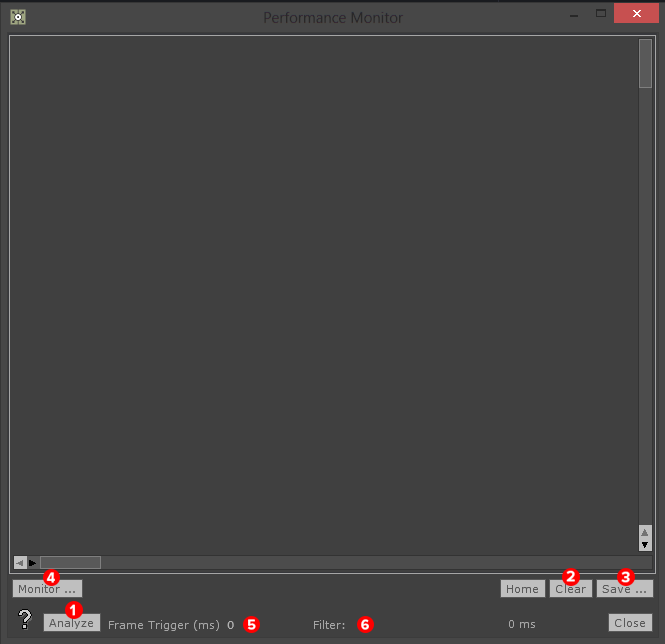
\includegraphics[width=11.5cm]{./img/11.3/performance-monitor-1.png}
\end{center}

\begin{enumerate}
\item Performs an analyses on the current frame
\item Clears the current results
\item Saves the current results to a text file
\item Change what is being monitored
\item A millisecond threshold value, which if crossed by a frame's cook time, will trigger the Performance Monitor to analyze
\item Filter the results for more precision, i.e. only CHOPS, TOPs, etc
\end{enumerate}

It is important to note that cook times are based on the CPU. This doesn't mean GPU bottlenecks will go unnoticed in the Performance monitor, but be cognizant that these are CPU readings. 

Here is an example analyses from the Performance Montior.

\begin{center}
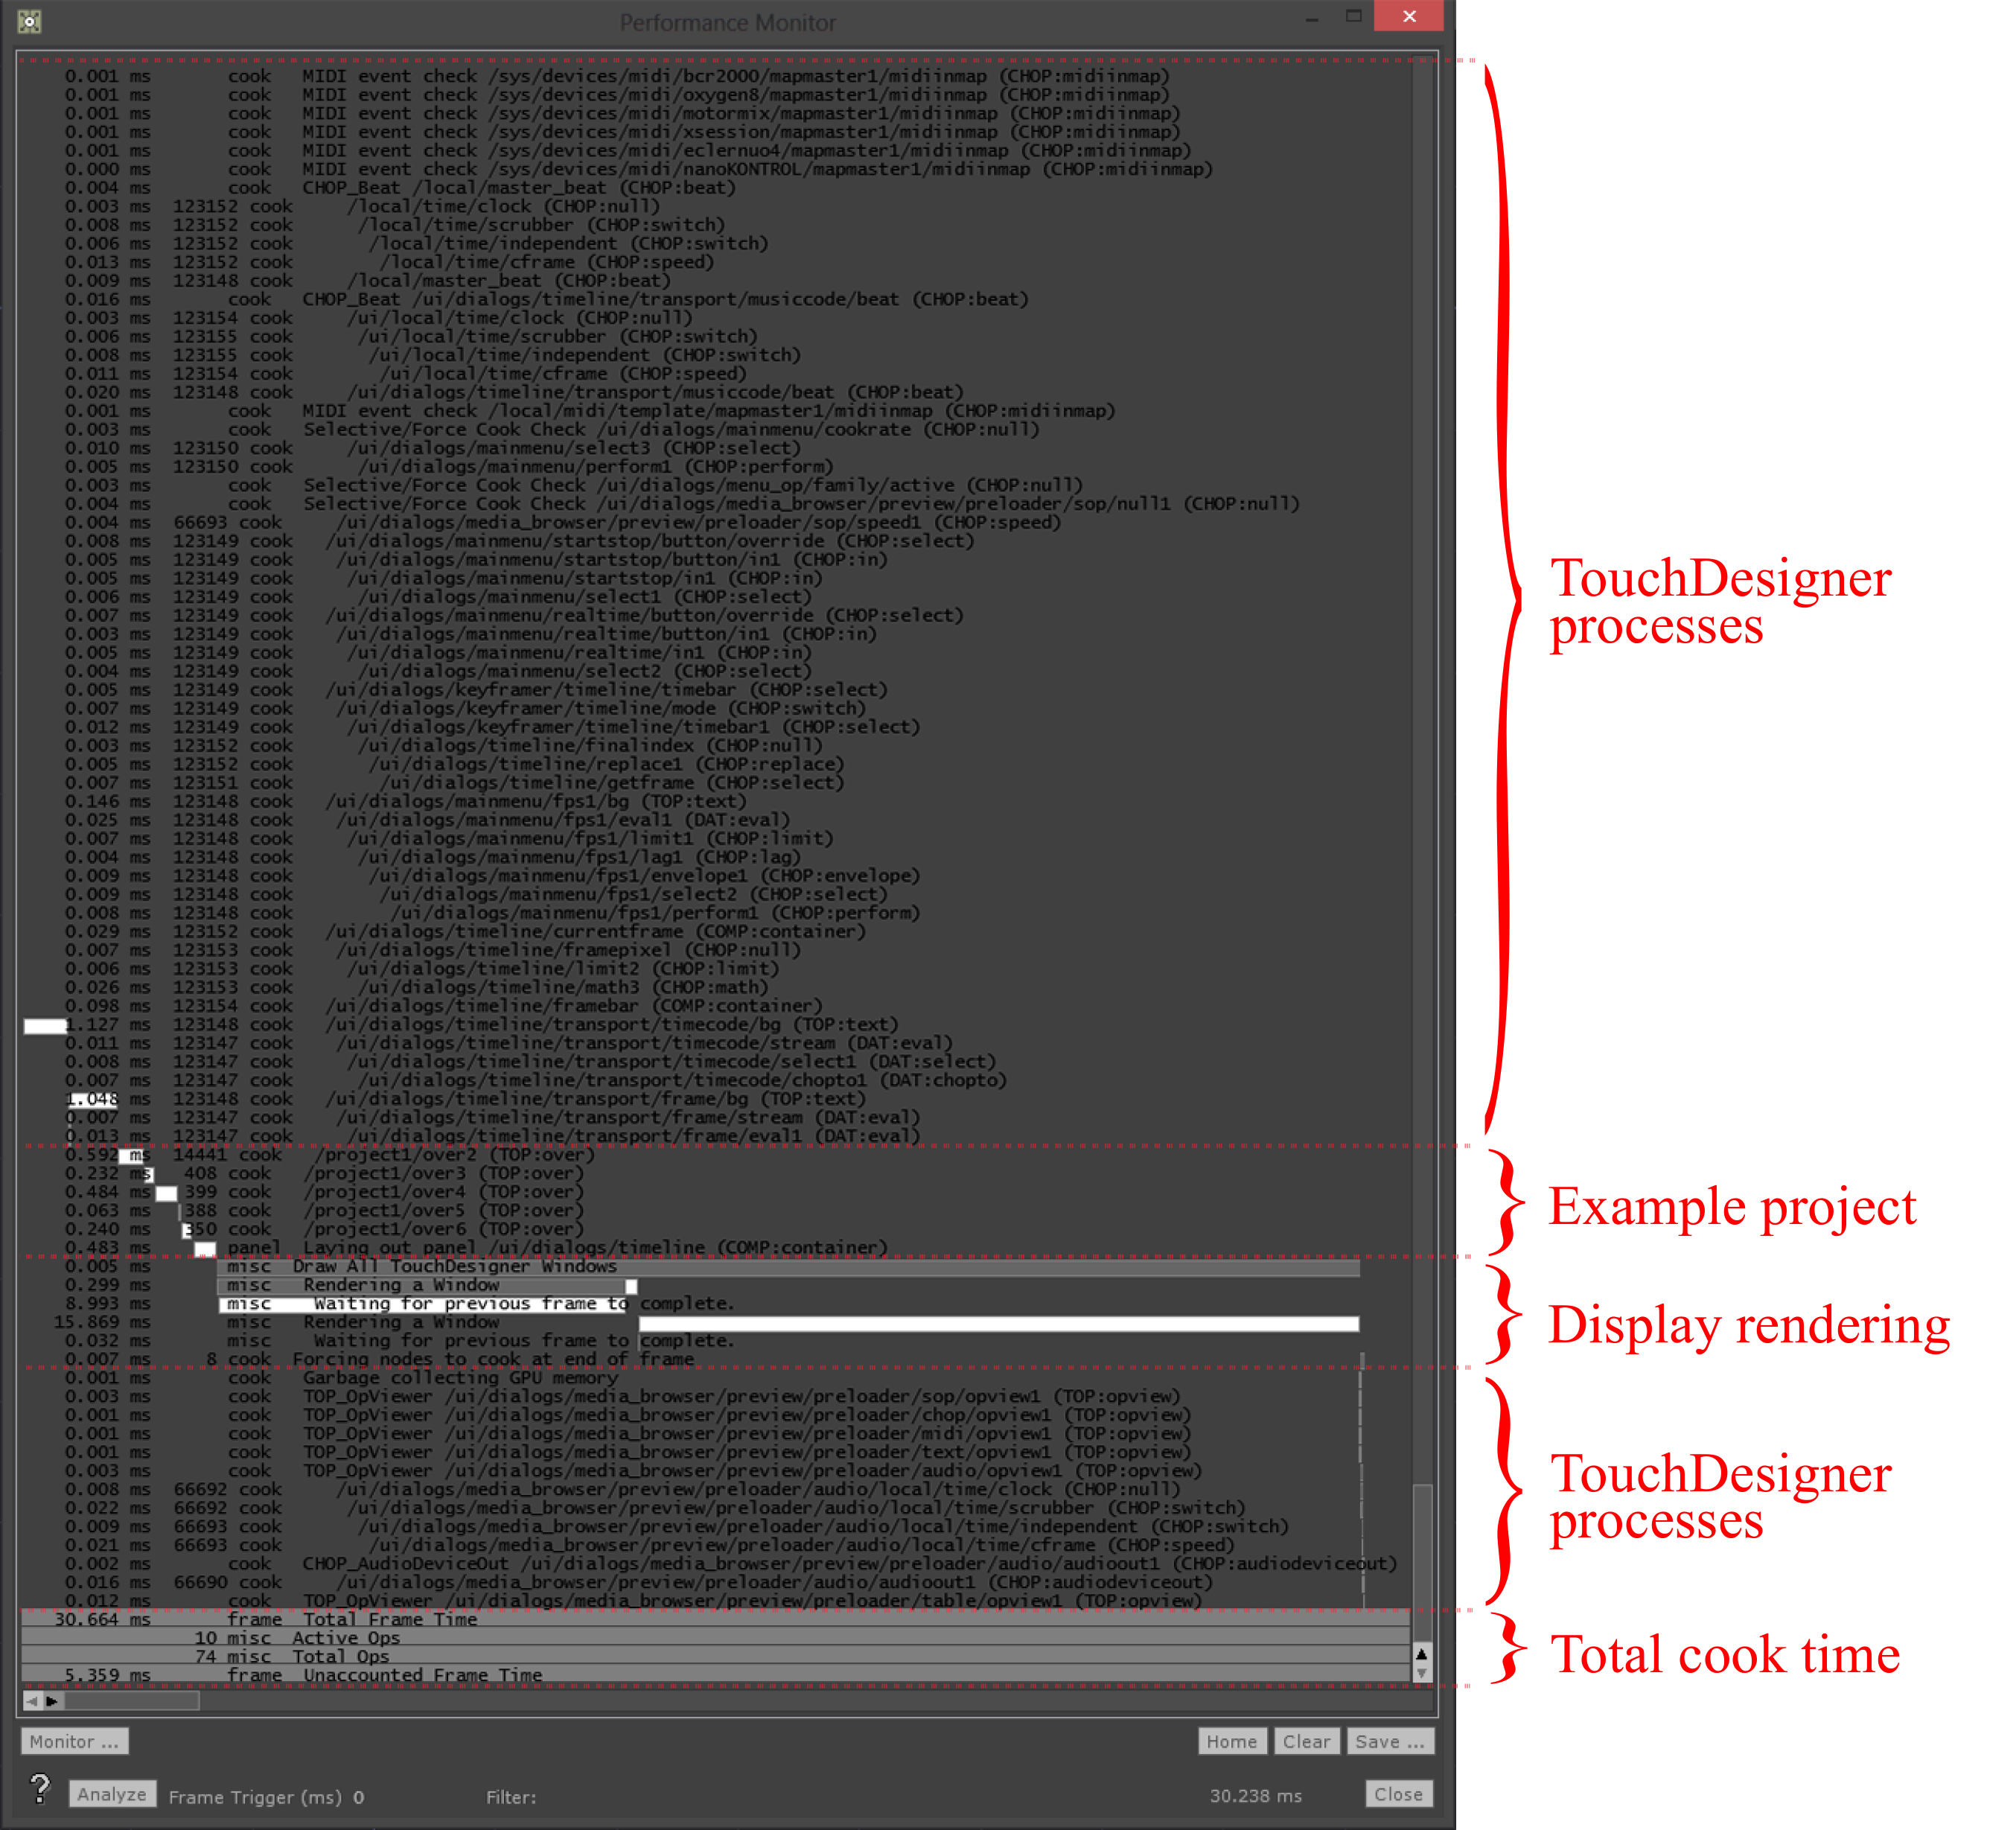
\includegraphics[width=14cm]{./img/11.3/performance-monitor-2.png}
\end{center}

The analyses above is taken from a simple project with a few Movie In TOPs and a few Over TOPs. Every frame that is analyzed will have some similar Operators. These are the Operators responsible for the functionality and user interface elements of TouchDesigner.

Look at the marked sections on the above diagram to see the cook times, and paths, for the Operators responsible for TouchDesigner's main functionality (User interfaces, dialog windows, etc), and more importantly the Operators belonging to the example project. The cook time of each Operator is represented by a white bar that is sized proportionally based on its contribution to the total cook time of that frame. When projects grow and become more involved, the section labeled 'Example project' will grow to include all of the project's Operators. This allows the analysis of a project to find problem Operators that too many system resources. 

In this example, the paths and cook times of the series of Over TOPs can be traced. They are all located inside of the 'project1' container, and their cook times range from 0.06 milliseconds to 0.6 milliseconds.  

A cautious side-note: Be careful of the effects of Vertical Sync and how cook time is perceived in the Performance Monitor. The graphics card will try to lock project FPS and display refresh rate. At 30 FPS, even in an empty project, the cook time per frame might be perceived as 33 milliseconds. The same effect can occur when working at 60 FPS, except that the Performance Monitor would show a frame cook time of 16 milliseconds. This doesn't mean that each frame actually needs a full 33 ms or 16 ms to render a frame, but that Vertical Sync is trying to sync TouchDesigner's FPS and the refresh rate of the displays. 

\end{fullwidth}

%------------------------------------------------

\section{Operator Cooking}

\begin{fullwidth}
Better performance can always be achieved by decreasing the amount of Operators that cook every frame. Many beginners never take this into account when creating Networks. Admittedly, everyone has worked on prototypes with tight deadlines, and has had to created Networks without much foresight. However, not taking cooking into account can be quite hazardous if a project can't afford any dropped frames.

The main goal is to perform static operations as early as possible in the signal flow, to prevent those specific from being rendered every frame.

Open example 'Cooking\_1.toe'. In this example, there is a simple graphic that rotates, and then various Operators are used to give the image a more interesting look. A feature that can help with optimizing Networks is the animation of the wires connecting Operators. Animated wires mean that the Operators on both ends are being cooked every frame. Starting at the far left of the Network, the wire between the Movie In TOP and the Transform TOP is not animated. This is because the image is loaded, and remains static. Operators only cook when they need to perform an operation or change. A still picture is static, and therefore does not change, and does not cook every frame. 

On the contrary, the rest of the wires in the Network are animated, meaning that everything after the Movie In TOP is cooking every frame. For this project, this isn't a dire problem, because there isn't anything extremely complex happening. Getting in the mind set of making efficient Networks from the start can save a lot of headaches come performance time. Let's take a look at this project in the Performance Monitor. 

\begin{center}
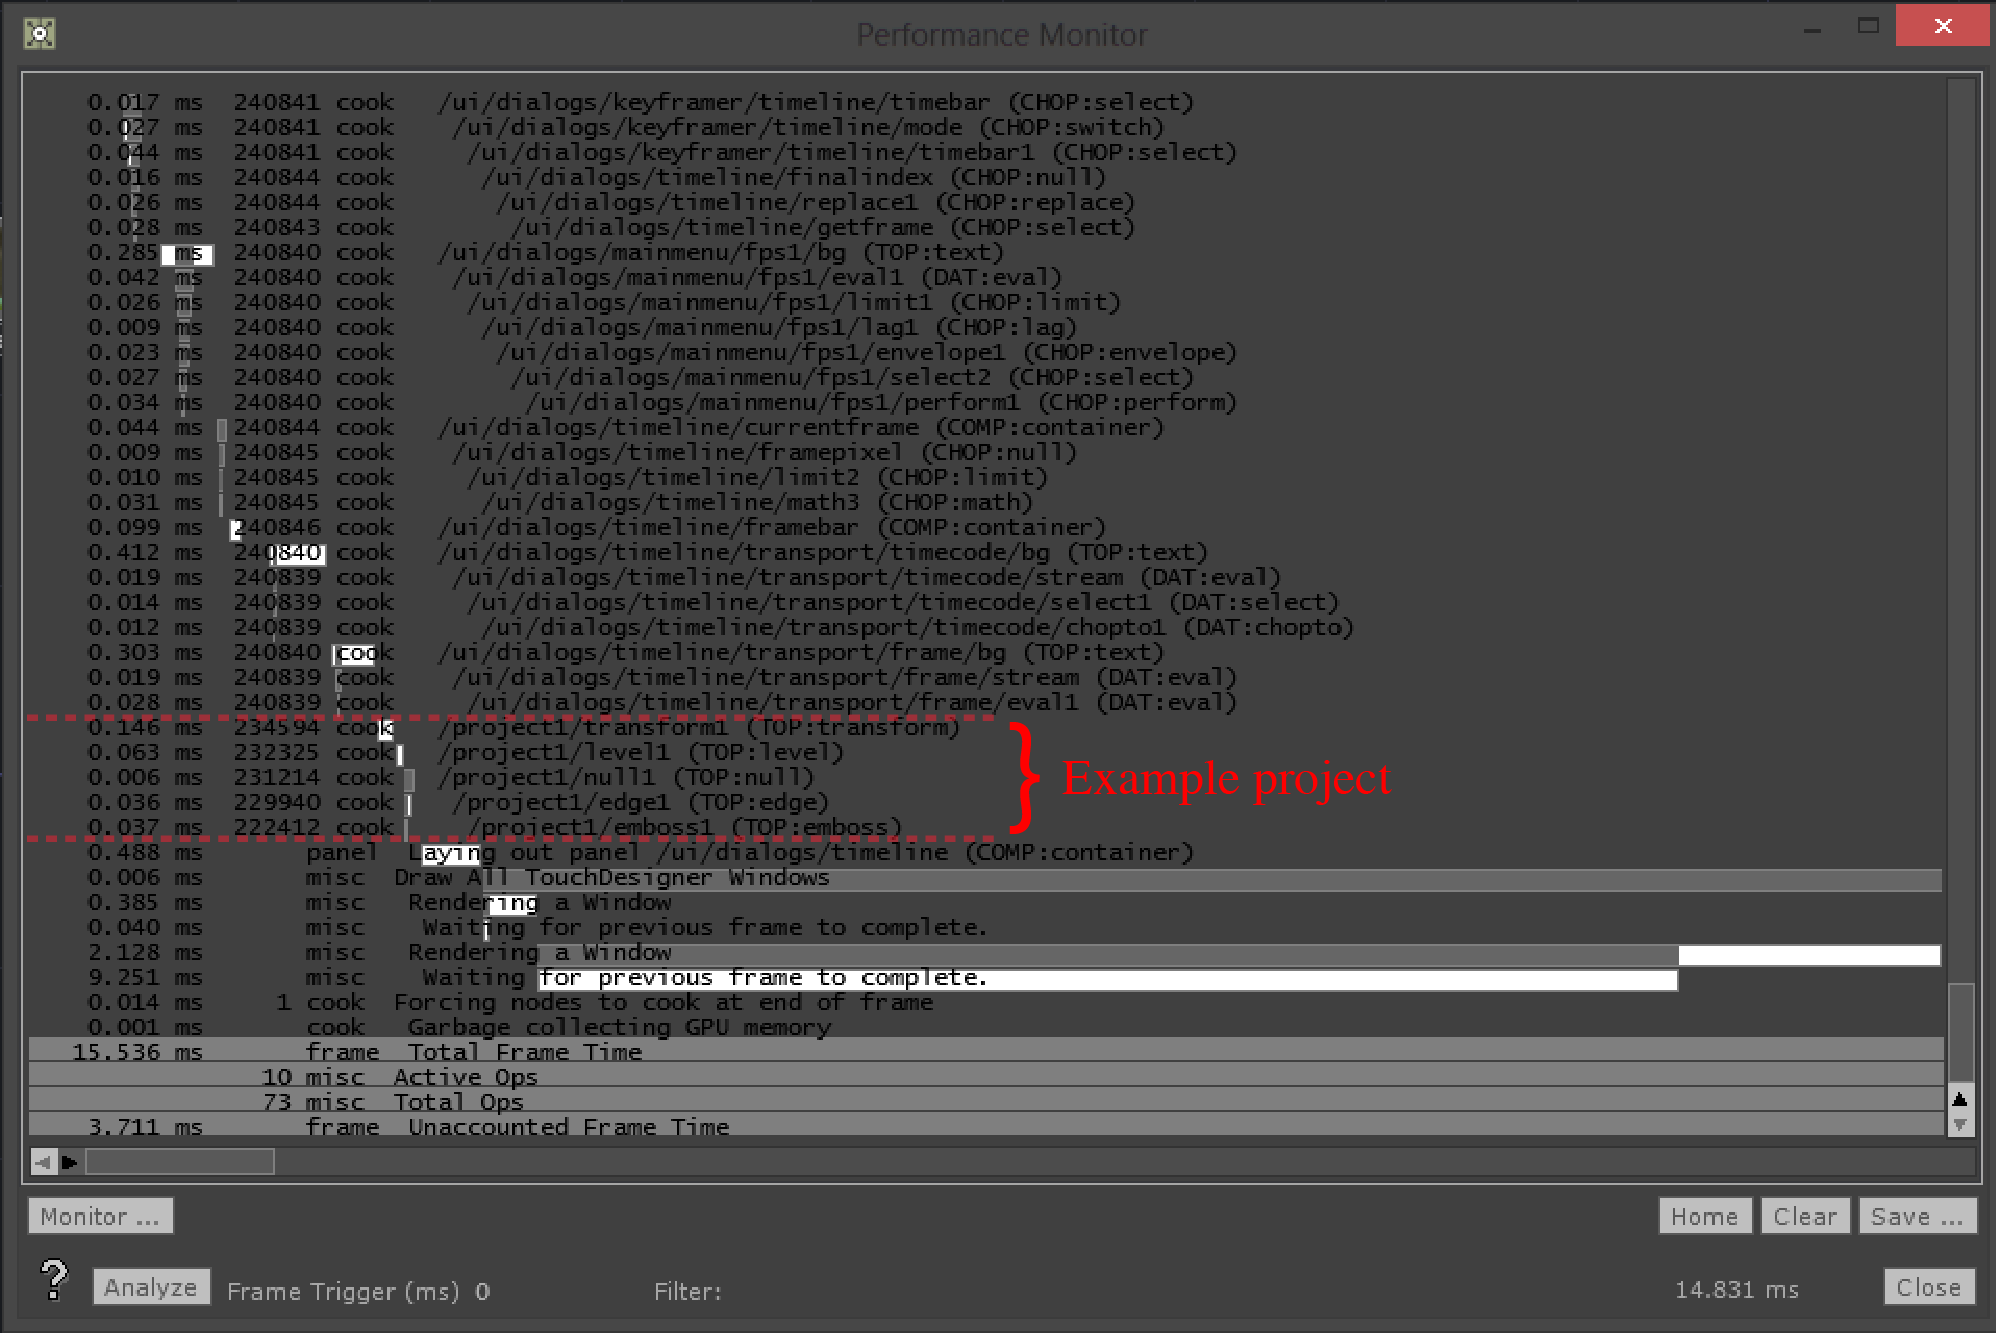
\includegraphics[width=12cm]{./img/11.4/operator-cooking-1.png}
\end{center}

Ignoring all the Operators needed for TouchDesigner's functionality, there is a small block of Operators dedicated to this example. The operations being performed on the image, in total, take about 0.25 milliseconds. As mentioned, static operations only need to cook once, and something to note is that many of the operations after the Transform TOP are  static in nature. Let's re-arrange these and see the gains in performance.

Open example 'Cooking\_2.toe'. This project is the same as the previous, except the Operators have been re-arranged. Before examining the signal flow closer, let's take a look at the Performance Monitor.

\begin{center}
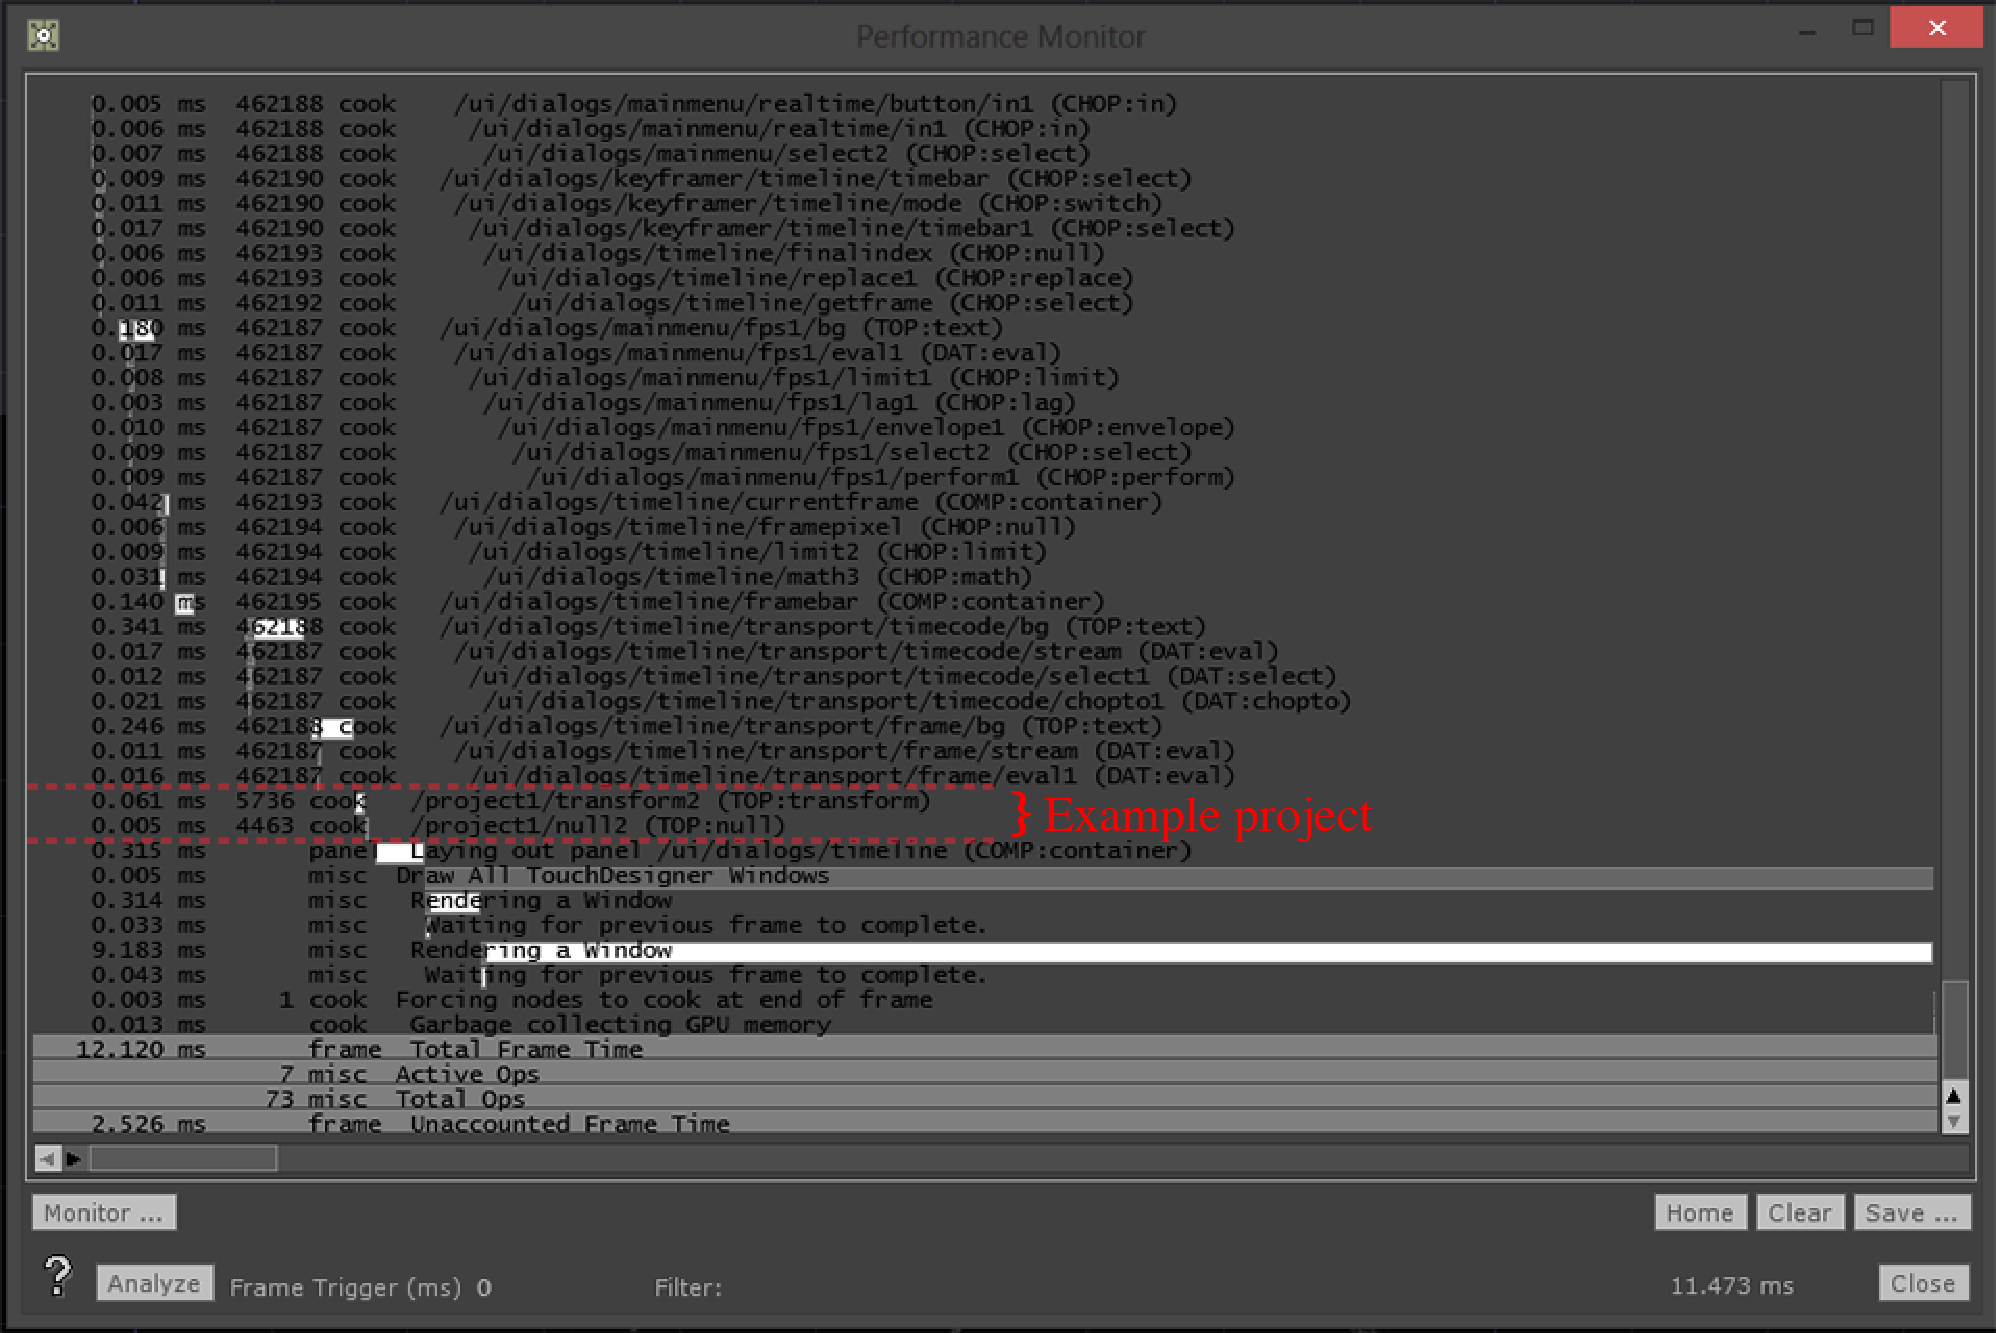
\includegraphics[width=12cm]{./img/11.4/operator-cooking-2.png}
\end{center}

At first glance it appears as if the project has shrank! A few of the Operators that were listed previously have disappeared. This is because these Operators aren't cooking every frame. In the last example, the Transform TOP was performing a transformation every frame, forcing the TOPs after it to recalculate their operations every frame. In this example, all of the static operations happen at the start of the signal flow, leaving the Transform TOP free to perform its transformation, without forcing any other Operators to recalculate their operations, or cook.

Taking a more in depth look at the Performance Monitor reading, the only Operator that was cooked was the Transform TOP, which took 0.061 milliseconds to cook. Compare this to the previous example, where the series of operations took 0.25 milliseconds to cook. That is an unbelievable gain for such a simple change.

It is worth noting that side by side, the outputs of these two Operator chains may not be exactly identical, but they are so indistinguishable from each other that many clients and artists will not mind the difference, knowing that the massive performance gains will allow them to do so much more.

\end{fullwidth}

%------------------------------------------------

\section{Resolution}

\begin{fullwidth}

When it comes to working with 2D textures, resolution is extremely important, because of the almost 1:1 ratio of pixels processed compared to processing power used.

An incredibly easy way to demonstrate this fact is through example. Open example 'Resolution\_1.toe'. This is a simple setup. The butterfly is composited on a bigger canvas, then using some LFOs, the opacity and blur are modulated before it is composited onto the forest background.  Middle clicking on any of the TOPs will reveal that this example requires just over 100MB of GPU RAM. That's not a lot of memory on a system with 4+ GB of GPU RAM, but this can quickly add up. Try to composite 40 of these butterflies in real-time, and 4GB can easily be spent. 

Now contrast this to example 'Resolution\_2.toe'. It creates the exact same results, but for only 60MB of GPU RAM. That is a significant difference. Take the above example of compositing 40 butterflies, and using this second method, only about 2.4 GB of GPU RAM are needed. All of the extra headroom from a simple change in resolution. The source butterfly asset is only 512x512 pixels, and in the first example, it is immediately composited on a 1920x1080 pixel canvas that is modulated. This creates a scenario where TouchDesigner is constantly re-drawing all 1920x1080 pixels every frame that the butterfly is modulated. 'Empty' pixels that have neither colour or alpha data are also re-drawn. In the second example, the exact same operations are being performed, but only on the source asset, which is a much lower resolution. This modulated asset is then composited on the 1920x1080 canvas. This saves the GPU having to re-draw a large canvas of pixels, when only a small section requires processing, thus saving quite a bit of GPU RAM and processing power.

\end{fullwidth}

%------------------------------------------------

\section{GPU Memory Fragmentation}

\begin{fullwidth}

Operators that use the GPU will often allocate the resources required for their tasks, and hold onto them until the task has been completed or changed.

GPU Fragmentation is one of the main concerns when working working with projects that have many different content sources. For example, a Constant TOP with a resolution of 1280x720 is connected to 10 other Operators. Once connected and cooked, each Operator will set aside the proper amount of GPU memory required to handle the processing of its specific amount of pixels. Once the memory is allocated, the Operators can operate relatively efficiently within their allocated space.

If the resolution of the source Constant TOP is changed, this will trigger a chain reaction, where all of the 10 other Operators will have to reallocate the correct amount of GPU resources for their tasks. If the Operator's resources are reallocated efficiently, many of the same memory blocks will be reused. If on the off-chance they can't reuse memory blocks, they'll have to relocate to the end of the memory. If this happens enough times in quick succession, the GPU memory will be fragmented, leaving the project in a state of poor performance while the GPU tries to defragment it's memory.

The two diagrams below try to outline memory fragmentation in the simplest way possible.

There are two case studies, both with similar parameters: There are 3GB of GPU RAM and there are three 1GB static textures to load and hold in RAM indefinitely.

\begin{center}
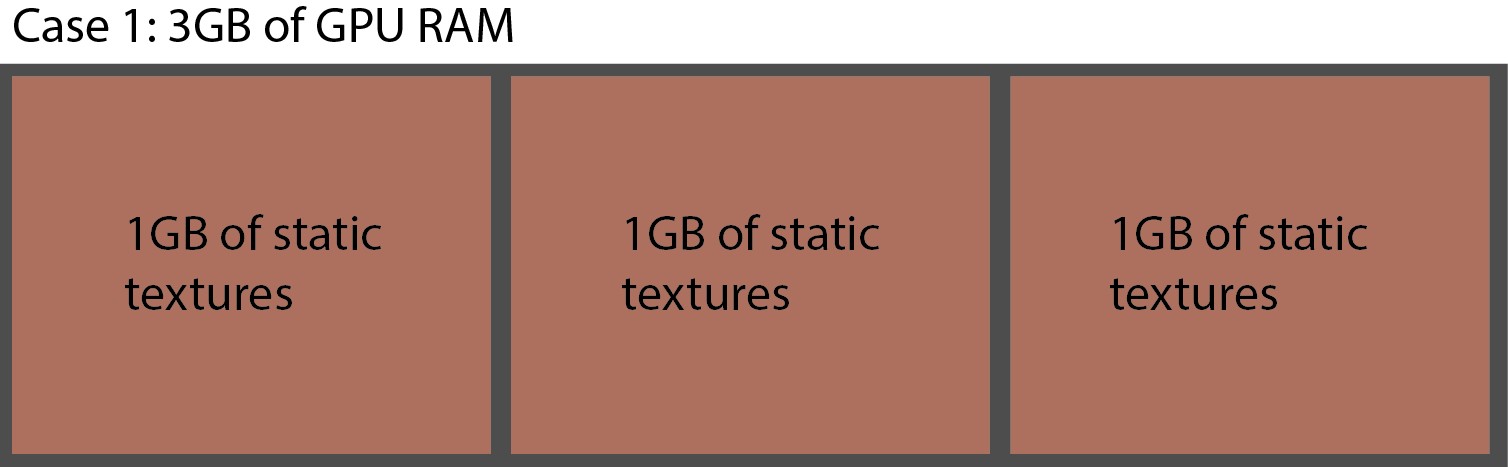
\includegraphics{./img/11.6/memory-frag-1.png}
\end{center}

In Case 1, the 3GB GPU of RAM would be able to perfectly fit the three 1GB static textures. They are called static textures because once they've allocated to memory, they aren't changed. This is the equivalent to loading a large image into a Movie In TOP at the start of a project and leaving it there indefinitely.

This is a perfect world situation, as there are many other processes that use GPU RAM, meaning resources are constantly in flux, and there would never be 3GB of free RAM on a graphics card that only has 3GB of GPU RAM.

Case 2 describes a situation where memory fragmentation will occur. To the already existing three 1GB textures, a 200MB texture is added to the mix. In this example, the loading and unloading is to happen in the following order:

\begin{enumerate}
\item Load 1GB texture
\item Load 200MB texture
\item Load 1GB texture
\item Unload 200MB texture
\item Load 1GB texture
\end{enumerate}

This would simulate a situation where a texture is loaded, displayed, and then replaced with another texture. 

\begin{center}
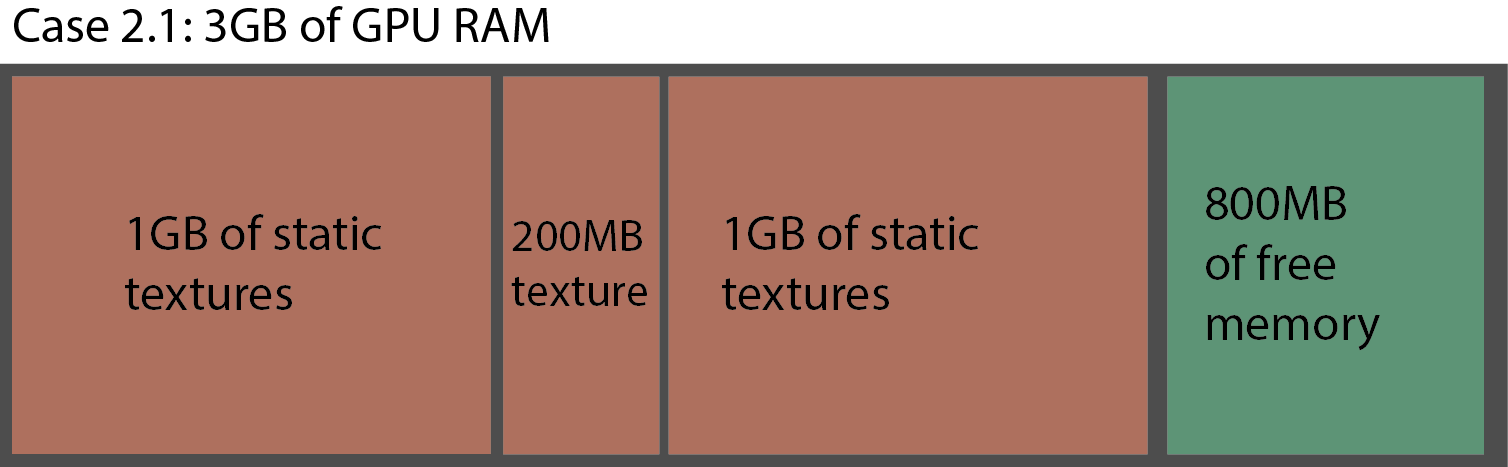
\includegraphics{./img/11.6/memory-frag-2.png}
\end{center}

In diagram 'Case 2.1', Steps 1 through 3 are completed, and there is 800MB free. At first glance, this might seem perfect, because if the 200MB texture is unloaded, there would be 1GB of free space for the final texture. Unfortunately, this isn't how graphics cards work.

\begin{center}
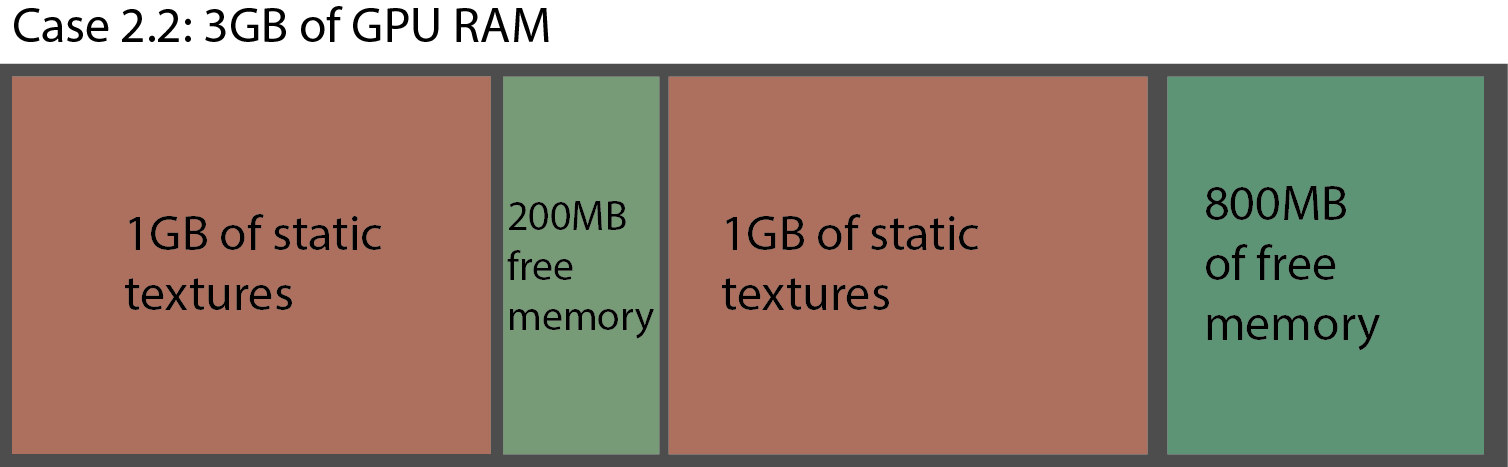
\includegraphics{./img/11.6/memory-frag-3.png}
\end{center}

As seen above, in diagram 'Case 2.2', Step 4 has been completed, and the 200MB texture has been unloaded. What remains is a prime example of GPU memory fragmentation. There is a total of 1GB of free GPU memory, but there isn't a single block of 1GB to allocate to the 1GB texture. The already-loaded 1GB textures, in their static state, can't be shifted in the GPU memory without a full unload and reload process occurring, and because the memory can't be shifted, the 200MB of free space has been trapped between the static textures. This 200MB allocation can be filled with 200MB or smaller textures, but it will not be able to load the third 1GB static texture.

The best way to prevent heavy memory fragmentation is to try to and restrict the amount of varying resolutions in a project. When an asset is swapped out for one that is the same resolution, often times it can take it's place in the memory.

\end{fullwidth}

%------------------------------------------------

\section{Windows System Processes}

\begin{fullwidth}
Windows is a complex operating system, and there are many processes and system-related applications running behind the scenes. Many of these processes and applications can negatively impact performance of a computer, and TouchDesigner. 

Windows is made for a large market of consumers, who primarily use their computers during the day. Because of such, there are many applications and Windows system operations that are scheduled to run if a computer is left powered-on overnight. This can be problematic for performance installations that run 24 hours a day. Depending on the needs of the installation or performance, many different applications and system related tasks can, and should, be turned off and rescheduled.

Applications such as virus and spyware scanning softwares, albeit useful for daily computing, should generally be avoided when using TouchDesigner. Virus and spyware softwares can cause a number of issues, the first being pop-ups. Many of these softwares display pop-up reminders and notifications at regular intervals. In unfortunate situations, these can overlap with displayed content and cover outputs during performances and installations. These applications can negatively effect the hard drive as well, as they often scan the system for viruses and malware, using up hard drive read \& write cycles. These two issues are aside from the CPU toll that many of these ever-running applications can incur. 

\end{fullwidth}